% \pgfplotsset{width=7cm,height=3cm,compat=1.10}
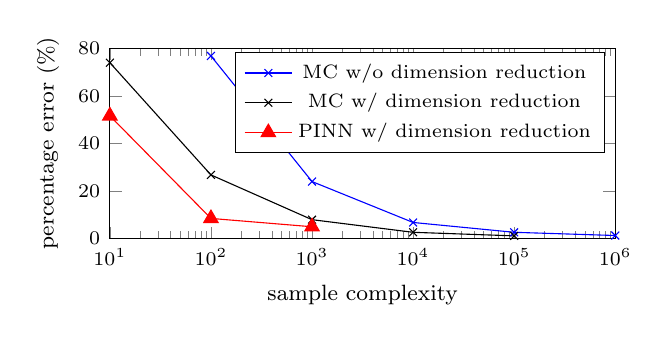
\begin{tikzpicture}
\begin{axis}[
    % x=0.5cm,
    % y=0.5cm/10,
    xlabel=\footnotesize{sample complexity},
    ylabel=\footnotesize{percentage error (\%)},
    xmode = log,
    xmin=10, xmax=10^6,
    ymin=0, ymax=80,
    % xtick={10^2,10^4,10^6},
    ytick={0,20,40,60,80},
    width=8cm,height=4cm,
    font = \scriptsize, 
            ]
\addplot[mark=x,blue] plot coordinates {
    (10^2,100*0.7675)
    (10^3,100*0.2399)
    (10^4,100*0.0680)
    (10^5,100*0.0267)
    (10^6,100*0.0132)    
};
\addlegendentry{MC w/o dimension reduction}

\addplot[color=black,mark=x,black]
    plot coordinates {
        (10^1,100*0.7392)
        (10^2,100*0.2678)
        (10^3,100*0.0797)
        (10^4,100*0.0267)
        (10^5,100*0.0117)
    };
\addlegendentry{MC w/ dimension reduction}

\addplot[color=red,mark=triangle*, mark size=3pt]
    plot coordinates {
        (10, 51.6)
        (100, 8.5)
        (1000,5)
    };
\addlegendentry{PINN w/ dimension reduction}
\end{axis}
\end{tikzpicture}